\chapter{Конформационное поведение производных и гетероаналогов бицикло[3.3.1]нонана (обзор литературы)}

Конформационный анализ молекулярных структур часто включает их разбиение на~подструктуры с дальнейшим выражением конформации структуры в~целом как суперпозиции конформаций подструктур. Система бицикло[3.3.1]нонана допускает несколько подобных разбиений~(рис.~\ref{fig:Decomposition:331}):

\begin{enumerate}
\item\label{item:331:Decomposition:6:6} Два 1,3-конденсированных шестичленных цикла (здесь и~в~дальнейшем циклы будем обозначать вместе с~направлением обхода): $\text{\CycleFirst} = \left(1\rightarrow 2\rightarrow 3\rightarrow 4\rightarrow 5\rightarrow 9\right)$ и~$\text{\CycleSecond} = \left(5\rightarrow 6\rightarrow 7\rightarrow 8\rightarrow 1\rightarrow 9\right)$;
\item\label{item:331:Decomposition:8:1} Восьмичленный цикл~$\text{\CycleThird} = \left(8\rightarrow 7\rightarrow 6\rightarrow 5\rightarrow 4\rightarrow 3\rightarrow 2\rightarrow 1\right)$ с одноатомным мостиком $\cdots9\cdots$ между положениями 1 и 5;
\item\label{item:331:Decomposition:2x2:2} Три взаимодействующих трёхатомных фрагмента: $2-3-4$, $8-7-6$ (т.\,н. \tqt{крылья}) и $1-9-5$;
\end{enumerate}

\begin{figure}
\centering
\begin{tabular}{|c|c|c|}
%\toprule
\multicolumn{3}{c}{\chemfig{[:-30,1.25]9*6(-1(-[:180]2-[:120]3-[:+60]4-[:0]\phantom{5}?)-8-7-6-5-)}} \\
\multicolumn{3}{c}{\cmpd{Bicycle331} } \\
%\midrule
\ref{item:331:Decomposition:6:6} & \ref{item:331:Decomposition:8:1} & \ref{item:331:Decomposition:2x2:2} \\
\chemfig{[:-30]3?-[:-60]2-[:0]1-[:+120]9-[:+60]5-[:+180]4?}\chemfig{[:-30]9*6(-1-8-7-6-5-)} &
\chemfig{[:-30]9*6(-[,,,,dash pattern=on 1pt off 1pt]1(-[:180]2-[:120]3-[:+60]4-[:0]\phantom{5}?)-8-7-6-5-[,,,,dash pattern=on 1pt off 1pt])} & 
\chemfig{[:-30]9*6(-1(-[:180,,,,dash pattern=on 1pt off 1pt]2-[:120]3-[:+60]4-[:0,,,,dash pattern=on 1pt off 1pt]\phantom{5}?)-[,,,,dash pattern=on 1pt off 1pt]8-7-6-[,,,,dash pattern=on 1pt off 1pt]5-)} \\
$\leftarrow$\qquad$\longleftarrow$ & $\longrightarrow$ & \\ 
%\bottomrule
\end{tabular}
\vspace{\bigskipamount}
\caption{\label{fig:Decomposition:331} Номенклатура положений и подструктурные декомпозиции системы бицикло[3.3.1]нонана}
\end{figure}

Конформация данного бициклического скелета традиционно определяется согласно разбиению~\ref{item:331:Decomposition:6:6}, т.\,е. из двух составляющих его конформаций шестичленных циклов~(рис.~\ref{fig:Conformations:Six}). Для насыщенных производных выделяются конформации \tqt{двойное кресло}~(\CC{}), \tqt{ванна-кресло}~(\BC{}), \tqt{кресло-ванна} (\CB{}), \tqt{кресло-ванна}~(\CB{}) и~\tqt{двойной ванны} (\BB{})~(рис.~\ref{fig:System331:379XYZ:Conf}). В случае структурной эквивалентности \tqt{крыльев} наблюдается \emph{конформационное вырождение} "--- формы \CB{} и \BC{} становятся структурно и~энергетически неразличимыми.

\begin{figure}
  \centering
  \begin{tabular}{rccc}
    &\chemfig{?-[:-150,0.75]<[:-30,0.75]-[:+30,1.5,,,line width=\boldbondwidth]>[:-30,0.75]-[:-150,0.75]?} &
    \chemfig{(-[:-35]?)<[:-60]-[:+0,1.5,,,line width=\boldbondwidth]>[:+60]-[:-145]?} &
    \chemfig{?<[:-60]-[:+20,,,,line width=\boldbondwidth]>[:-20]-[:+120]-[:-160]?} \\
    &\ConfName{Т} & \ConfName{В} & \ConfName{К}\\
\CycleFirst: & \chemfig{X?-[:-150,0.75]<[:-30,0.75]-[:+30,1.5,,,line width=\boldbondwidth]Z>[:-30,0.75]-[:-150,0.75]?} &
    \chemfig{X(-[:-35]?)<[:-60]-[:+0,1.5,,,line width=\boldbondwidth]>[:+60]Z-[:-145]?} &
    \chemfig{X?<[:-60]-[:+20,,,,line width=\boldbondwidth]>[:-20]Z-[:+120]-[:-160]?} \\
\CycleSecond: & \chemfig{Y?-[:-150,0.75]<[:-30,0.75]-[:+30,1.5,,,line width=\boldbondwidth]Z>[:-30,0.75]-[:-150,0.75]?} &
    \chemfig{Y(-[:-35]?)<[:-60]-[:+0,1.5,,,line width=\boldbondwidth]>[:+60]Z-[:-145]?} &
    \chemfig{Y?<[:-60]-[:+20,,,,line width=\boldbondwidth]>[:-20]Z-[:+120]-[:-160]?} \\
  \end{tabular}
  \vspace{\medskipamount}
  \caption{\label{fig:Conformations:Six}Базисные конформации шестичленных циклов}
\end{figure}


\begin{figure}
\centering
\begin{tabular}{c|c}
\multicolumn{2}{c}{
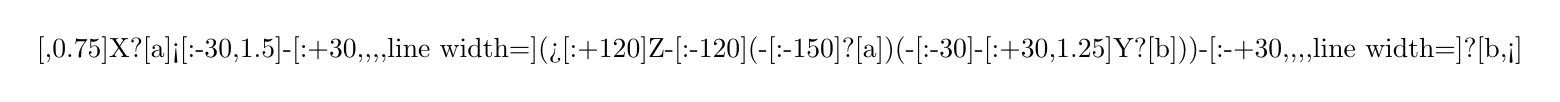
\begin{tikzpicture}
\node(Bicyclo331) at(0,0) {%
\chemfig{[,0.75]X?[a]<[:-30,1.5]-[:+30,,,,line width=\boldbondwidth](>[:+120]Z-[:-120](-[:-150]?[a])(-[:-30]-[:+30,1.25]Y?[b]))-[:-+30,,,,line width=\boldbondwidth]?[b,{<}]} };
\end{tikzpicture}
}
\\
\multicolumn{2}{c}{\BB{}~(\TT{})} \\
\midrule
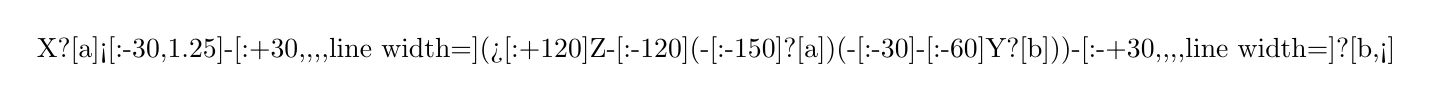
\begin{tikzpicture}
\node(Bicyclo331) at(0,0) {%
\chemfig{X?[a]<[:-30,1.25]-[:+30,,,,line width=\boldbondwidth](>[:+120]Z-[:-120](-[:-150]?[a])(-[:-30]-[:-60]Y?[b]))-[:-+30,,,,line width=\boldbondwidth]?[b,{<}]} };
\end{tikzpicture}
& 
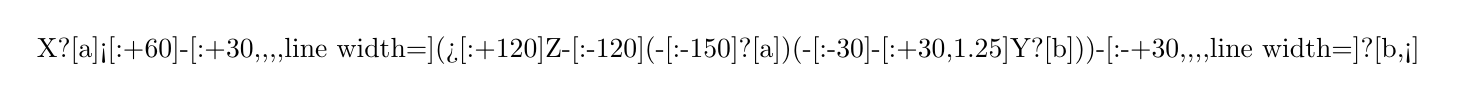
\begin{tikzpicture}
\node(Bicyclo331) at(0,0) {%
\chemfig{X?[a]<[:+60]-[:+30,,,,line width=\boldbondwidth](>[:+120]Z-[:-120](-[:-150]?[a])(-[:-30]-[:+30,1.25]Y?[b]))-[:-+30,,,,line width=\boldbondwidth]?[b,{<}]} 
};
\end{tikzpicture}
\\
\BC{} & \CB{}
\\
\midrule
\multicolumn{2}{c}{%
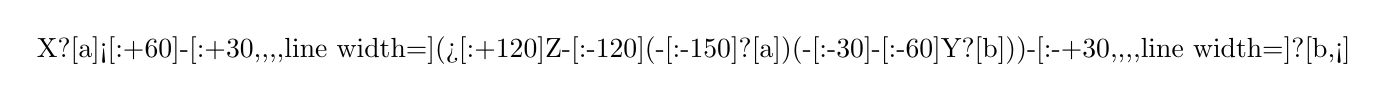
\begin{tikzpicture}
\node(Bicyclo331) at(0,0) {%
\chemfig{X?[a]<[:+60]-[:+30,,,,line width=\boldbondwidth](>[:+120]Z-[:-120](-[:-150]?[a])(-[:-30]-[:-60]Y?[b]))-[:-+30,,,,line width=\boldbondwidth]?[b,{<}]} 
};
\end{tikzpicture}
}
\\
\multicolumn{2}{c}{\CC{}}
\\
\end{tabular}
\caption{\label{fig:System331:379XYZ:Conf}Основные конформации 3X,~7Y,~9Z-аналогов бицикло[3.3.1]нонана}
\end{figure}

Для пространственных форм насыщенных шестичленных циклов оптимальной является структура \tqt{кресла}~(\ConfName{К}); форма \tqt{ванна}~(\ConfName{В}) обычно является переходным состоянием в процессе пседовращения между двумя конформерами с \tqt{твист}-структурой~(\ConfName{Т}). Причиной этого признано сильное повышение энергии структур с ординарными связями в заслонённой конформации (так называемое \emph{питцеровское напряжение}). По этой же причине форма \BB{} у~производных бицикло[3.3.1]нонана встречается очень редко (характерна для сильно затруднённых и напряжённых молекул), и в этих случаях обычно наблюдается экспериментально в виде формы «двойного твиста» (\TT{}).

Торсионные напряжения также являются фактором устойчивости и для формы \CB{}, содержащей подструктуру \tqt{ванны}, в которой, однако, заслонённые конформации связей незначительно отклоняются от идеальной формы \ConfName{В} с эндоциклическими двугранными углами $\tau_{9123}\simeq 0$ и $\tau_{9543}\simeq 0$. Часто эти отклонения симметричны, т. е., $\tau_{9123} = - \tau_{9543}$. Всё это является, в частности, показателем стереохимической (конформационной) жёсткости формы \tqt{кресла} насыщенного шестичленного цикла. Такая жёсткость образуется из сочетания низкой энергии и высоких собственных частот колебания структуры. Жёсткие конформации одной из подструктур молекулы могут стабилизировать менее энергетически выгодные формы других как термодинамически, так и кинетически.

Конформация \CC{} состоит из кресловидных шестичленных циклов, почти свободных от питцеровского напряжения. Основным фактором устойчивости для этой конформации оказывается невалентное взаимодействие между \tqt{крыльями} бициклической системы. Особенно значима в этом смысле роль положений 3 и 7. Дисперсионное или электростатическое отталкивание между этими положениями или эндо-заместителями в них приводит к повышению энергии и дестабилизации \CC{} относительно других форм, тогда как притяжение стабилизирует соответствующую структуру.

Максимальная симметрия бициклического скелета~\cmpd{Bicycle331}, порождённая из~симметрической группы $\SymGroup{S}{9}$ как система комбинаторных циклов $\left\langle(1\,5)(2\,4\,6\,8)(3\,7)(9)\right\rangle$, изоморфно реализуется в мировом пространстве $\AGroup{E}^3\left(\AGroup{R}\right)\simeq\AGroup{R}^3$ в виде группы симметрии \(\SymGroup{C}{2v}\) для~\CC{} и~\BB{} и снижается до подгрупп для других конформаций: \(\SymGroup{C}{s}\) у~\CB{} и~\BC{}, $\SymGroup{C}{2}$ у~\TT{}.